%	----- PACKAGES AND OPTIONS ----- 
\documentclass[11pt,a4paper,english,oneside]{article}
\usepackage{etex} %Because of many packages --> Extended TeX.
\usepackage[left=1in, right=1in]{geometry} %Helps to structure the paper layout.
\usepackage[Lenny]{./style/fncychap} %Design of the thesis.
\usepackage[utf8]{inputenc} %Due to vowels.
\usepackage[british]{babel} %Define the language style.
\usepackage{dsfont} %Nice style for the indicator function.
\usepackage{fancyhdr} %To customize the headers and footers.
\usepackage{booktabs} %In case you need \cmidrule or \addlinespace in tables.
\usepackage[hang,bottom,stable,multiple]{footmisc} %Style of footnotes.
\usepackage{appendix} %For the \appendixpage command.
%Load some mathematical packages.
\usepackage{amsmath}
\usepackage{amsfonts}
\usepackage{amsmath}
\usepackage{amssymb}
\usepackage{mathtools}
\usepackage[sort,round]{natbib} %For the bibliography.
\usepackage{etoolbox} %To remove the page number on \appendixpage.
\usepackage{amsthm} %For theorems, definitions etc.
\usepackage{thmtools} %For theorems, definitions etc.
\usepackage{setspace} %Use double spacing.
\usepackage{lipsum} %For the \lipsum command to generate a text.
\usepackage{datetime} %For the specification of the date.
%\usepackage{tocloft} %The ToC, LoF and LoT each appear not necessarily on a new page.
\usepackage{graphicx,listings,xcolor,textcomp} %For the graphics, listings etc.
\usepackage[justification=raggedright,
            singlelinecheck=false,format=plain,
            font={large,bf},margin=10pt]{caption} %Customize the captions.
\usepackage{chngcntr} %To use counterwithout.
\usepackage{epstopdf} %For inserting .eps files into the document.
\usepackage{hyperref} %Must be loaded at the end.
\usepackage{xparse} %Load for \NewDocumentCommand command.
\usepackage{cleveref} %For the command \cref, load after hyperref.
\usepackage{arydshln} %Due to the capability to draw horizontal/vertical dash-lines.
\usepackage{array,hhline} %To create tables and matrices.
\usepackage{rotating} %To rotate a table.
\usepackage{tabularx} %An extended version of tabular.
\usepackage{pdfpages}

\graphicspath{ {./../resources/figures/} } %  Figures directory

%Setup of the reference links.
\hypersetup{
     colorlinks=false,
     linkcolor=blue,
     citecolor=blue,
     filecolor=magenta,
     urlcolor=blue}

%Define some reasonable margins.
\setlength{\textwidth}{6.6in}
\setlength{\textheight}{8.8in}
\setlength{\topmargin}{-0.1in}
\setlength{\oddsidemargin}{0in}
\setlength{\parskip}{1mm}

\bibliographystyle{abbrvnat} %Reference style.
\allowdisplaybreaks[1] %Page breaks of equations are allowed, but avoided if possible. 2-4 more relaxed.

%New command for the UZH logo.
\newcommand*{\plogo}{
\includegraphics{./style/uzh_logo_e_pos}}

%New command for the differential d to have an ordinary d.
\makeatletter
  \newcommand{\ud}{\mathrm{d}}
\makeatother

%Remove page number on \appendixpage. Use the package 'etoolbox'.
\makeatletter
\patchcmd{\@chap@pppage}{\thispagestyle{plain}}{\thispagestyle{empty}}{}{}
\makeatother

%Declare Definitions, Theorems etc.

%Readjust the numbering.
%\counterwithout{footnote}{chapter}
%\numberwithin{equation}{chapter}

\setlength{\parindent}{0cm} % Uncomment this if you don't want to have indents.

%	----- TITLE PAGE ----- 
\newcommand*{\titleGP}{\begingroup %Create the command for including the title page in the document.
\centering %Center all text.
\vspace*{\baselineskip} %White space at the top of the page.
\plogo\\[2\baselineskip] %University Logo.
\rule{\textwidth}{1.6pt}\vspace*{-\baselineskip}\vspace*{2pt} %Thick horizontal line.
\rule{\textwidth}{0.4pt}\\[\baselineskip] %Thin horizontal line.
{\LARGE Scarcity channel of Quantitative Easing :}

\vspace*{3pt}

{\LARGE Examining the Overnight Treasury Repo Market in the US}\\[0.2\baselineskip] %Title.
\rule{\textwidth}{0.4pt}\vspace*{-\baselineskip}\vspace{3.2pt} %Thin horizontal line.
\rule{\textwidth}{1.6pt}\\[2\baselineskip] %Thick horizontal line.
\scshape %Small caps.
Master's Thesis\\[2\baselineskip]
Submitted in partial fulfillment of the requirements for the degree of Master of Arts in Economics and Business Administration \par
\vspace*{2\baselineskip}
Author\\
{\Large Hubert Mrugala \\ [5pt]
 }
Seemattweg 4, 6315 Oberageri \\[5pt]
19-764-265 \\[5pt]
hubert.mrugala@uzh.ch \\


\vspace*{2\baselineskip}
Supervisor\\
{\Large Prof. Dr. Kjell Nyborg\\[5pt]\small Chaired Professor of Finance\\[5pt]
\small Department of Banking and Finance\\[5pt]University of Zurich\par}
\vspace*{2\baselineskip}
Assistant\\
{\Large Benjamin Schneider \par}
\vfill
{\scshape Date of Submission: 18.05.2022} \\[0.3\baselineskip]
\endgroup}

% ----- SPECIAL HEADER AND FOOTER STYLE  ----- 
% for the executive summary and Task Assignment section.
\fancypagestyle{firststyle}{%
  \fancyhf{}%
  \renewcommand{\headrulewidth}{0pt}
  \fancyfoot[C]{\thepage}}

%Customize headers and footers.
\pagestyle{fancy}
\fancyhead[R]{\thepage}
\fancyhead[L]{\rightmark}
\fancyfoot[L]{Hubert Mrugala}
\fancyfoot[C]{}
\fancyfoot[R]{Scarcity channel of Quantitative Easing}

%Define the signature line with dots.
\NewDocumentCommand \dotbox {o O{.5\linewidth} m O{3ex} O{\linewidth}}
{
  \begin{minipage}{7cm}
    \makebox[7cm][l]{\,.\dotfill}
    \\
    \makebox[7cm][l]{\,#3}
  \end{minipage}
}

% ----- BEGIN DOC AND PROJECT DEFINITION ----- 
\begin{document}

\thispagestyle{empty}
\titleGP
\newpage
\doublespacing
\setcounter{page}{1}
\pagenumbering{Roman}
\section*{Task Assignment}

\begin{figure}[h!]
  \begin{center}
    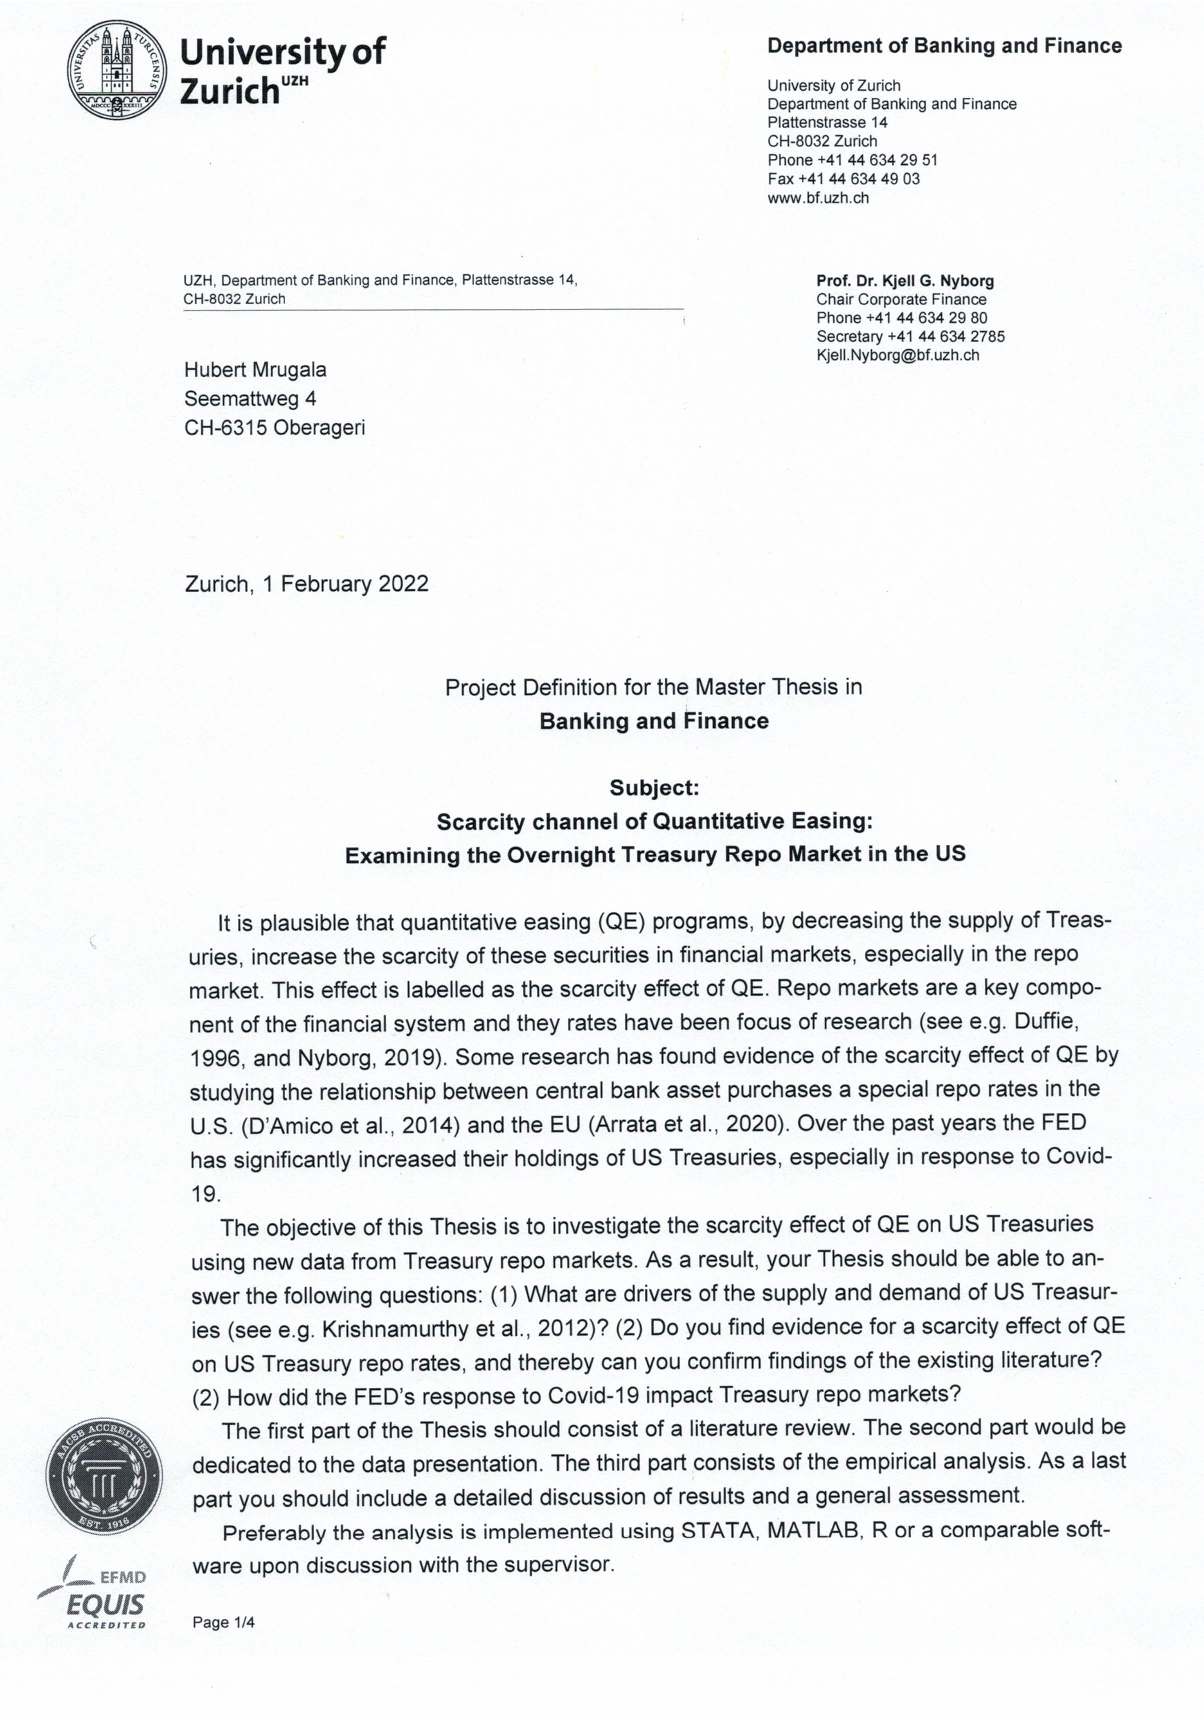
\includegraphics[page=1,width=.86\textwidth]{../../project_definition.pdf}
  \end{center}
\end{figure}
\newpage
\begin{figure}[h!]
  \begin{center}
    \includegraphics[page=2,width=.86\textwidth]{../../project_definition.pdf}
  \end{center}
\end{figure}
\newpage
\begin{figure}[h!]
  \begin{center}
    \includegraphics[page=3,width=.86\textwidth]{../../project_definition.pdf}
  \end{center}
\end{figure}
\newpage
\begin{figure}[h!]
  \begin{center}
    \includegraphics[page=4,width=.86\textwidth]{../../project_definition.pdf}
  \end{center}
\end{figure}

\thispagestyle{firststyle}
\newpage

% ----- EXEC SUMMARY AND ABSTRACT ----- 
\section*{Executive Summary}
\thispagestyle{firststyle}

\lipsum[1-3] % Here goes the text

\newpage
\tableofcontents
\newpage
\listoffigures
\newpage
\listoftables
\newpage
\pagenumbering{arabic}

\begin{center}
  {\Large \emph{\textbf{Scarcity channel of Quantitative Easing:\\
  Examining the Overnight Treasury Repo Market in the US}}}\\[4pt]
  Hubert Mrugala
\end{center}

\abstract{\lipsum[1]}

\begin{flushleft}
  \textbf{JEL classification}: E4, E5\\
  \textbf{Keyword}: Collateral, Scarcity, Treasury, Monetary Policy, Repo Market
\end{flushleft}

% ----- INTRODUCTION ----- 
\section{Introduction}

The COVID-19 pandemic has caused the deepest US recession since the Great Depression and induced the biggest monetary stimulus since the Global Financial Crisis. One of the monetary policy tools that was activated during the pandemic was an additional round of quantitative easing.\footnote{It was actually an acceleration of already present QE that was sparked by 2019 repo rumble.} In the time of 4 months, the Fed's balance sheet exploded from \$4.2 to \$7.1 trillion, and then kept growing. As of April 2022, total assets of the Fed reached almost \$9 trillion. Central bank asset purchases are used in normal times as a unconventional policy that helps achieving ultimate goals of the Fed, which are maximum employment and inflation level at 2\% over the longer run.

There are many theoretical transmission channels of quantitative easing, however almost all of those channels focus on positive effects of asset purchases. Negatives are very rarely analysed. \citet{nyborg2015} showed that collateral frameworks of ECB distort financial markets' efficiency by making bad collateral look better then it really is. What about a high-quality collateral? Can draining fist-class collateral out of the markets have an adverse impact on the economy?

There is one channel of quantitative easing that is rarely mentioned and insuffitiently studied.\footnote{In financial media, only Izabella Kaminska of FT Alphaville sometimes covered collateral scarcity.}. It is the scarcity channel (or scarcity effects). While most channels on QE focus on abundance of reserves, central bank liquidity, the scarcity effect, puts emphasis on the collateral-side of the swap, which is the public sector liquidity. There are only two academic papers that study the scarcity channel of asset purchases programmes. \citet{damico2014} find that there was a scarcity premium of US Treasury securities traded in the repo market during the time of LSAP programs. Likewise, \citet{arrata2018} determine a similar relationship in the \textbf{Euro zone market for repo contracts}. Both papers prove the existence of the scarcity effects in the US and EU markets, however, those investigations look only at specific special repo markets and don't take into account the mechanics of the collateral intermediation complex. Furthermore, there hasn't been any research done about the scarcity premium of US Treasuries in over eight years, despite an almost constant QE during that period.

This research fills the subject gap, the time gap, and the context gap in the narrow literature on scarcity effects. I use a General Collateral Financing Treasury Repo rate weighted index in a timespan of the last 15 years to test a connection between the level of US Treasury securities on the Fed's balance sheet and the index. Additionally, to focus completely on the collateral-side of a repo transaction, I use a collateral spread as a dependent variable just like \citet{nyborg2019b} does.

\textbf{[Findings]}

I control for \textbf{[...]} and emphasize the importance of high-quality collateral by describing its dynamics and economic function. Moreover, I add an innovative proxy for the re-use rate of collateral in the banking system as an extension of the base model.

The research connects three different strains of literature, which are research on collateral scarcity, repo markets and collateral intermediation.

Apart from already mentioned academic papers on scarcity effects, there is also one investigation of the Japanse JGB market that contributes to the literature on collateral scarcity. \han{2018} have documented that BoJ purchases of Japanese Government Bonds in QE and then QQE programs have negative impact on market liquidity, which suggest scarcity effects.

The second category is the literature on repo market rates and cash market rates of US Treasuries. The work of Duffie (1996) introduced a model that shows how short-selling Treasuries obtained by reverse-repo transactions can create squeezes at delivery dates and so, cause some repos to trade on special. Mark Fisher (2002) gives a nice example of how this often happens. Dealers short Treasuries, usually the kinds that show highest liquidity, to hedge their trading activities. At the same time, reverse-repo transaction (receiving collateral at initiation) is the most cost-effective way of getting necessary Treasuries. The result of this, is that the demand for these specific securities in the repo market rises substantially, while the supply is not sufficiently elastic. Hence, low special repo rates. Special repo rates are not planned to be studied in the proposed research, though the literature of this kind gives insight into supply-demand dynamics in the market. Moreover, US Treasury securities are special as a whole asset group. Just like in the case of the repo spread that determines the specialness of repos with specific Treasury collateral, Treasuries overall have a non-default component that makes them, in general, exceptional on their own (Krishnamurty and Vissing-Jorgensen 2012).

In the Euro area, repo markets are driven mainly by agents that seek collateral and not funding (Shaffner et al. 2019). Also, counterparty risk constrains make the quality of collateral in bilateral transactions crucial. If the collateral pledged is not safe or liquid enough, contracts will often be not agreed on (Ewerhart and Tapking 2008). After all, collateral side of the repo market may be more important than the financing side, which gives more arguments to study the effect of the central bank purchases on the repo market.

The last branch of literature is concerned with the collateral supply and its intermediation. Singh and Stella (2012) introduce and explain a phenomenon of "collateral-chains". Dealer banks get “source collateral” from hedge funds and securities lending custodians to use that collateral for their own purposes by repledging it (rehypothecation). This means that large banks will source the collateral from non-banks and pledge it in another transaction, then another bank receiving that particular collateral can also re-use it, and so a collateral-chain is created. A re-use rate, or velocity, of collateral shows how many times a source collateral has been pledged. Singh (2017) reports that the collateral re-use rate in 2007 was 3.0, and then it was continuously dropping to 1.8 \in 2015. Jank et al. (2020) found a positive relationship between ECB bond purchases (PSPP) and the re-use rate of collateral suggesting that the market participants adjust to shocks in collateral scarcity by utilizing more the source collateral.

This study is important because...

The remainder of the paper is organized as follows. 


\begin{figure}[htb!]
  \begin{center}
    \caption{Fed's Balance Sheet and 10-year US Treasury Yield}
    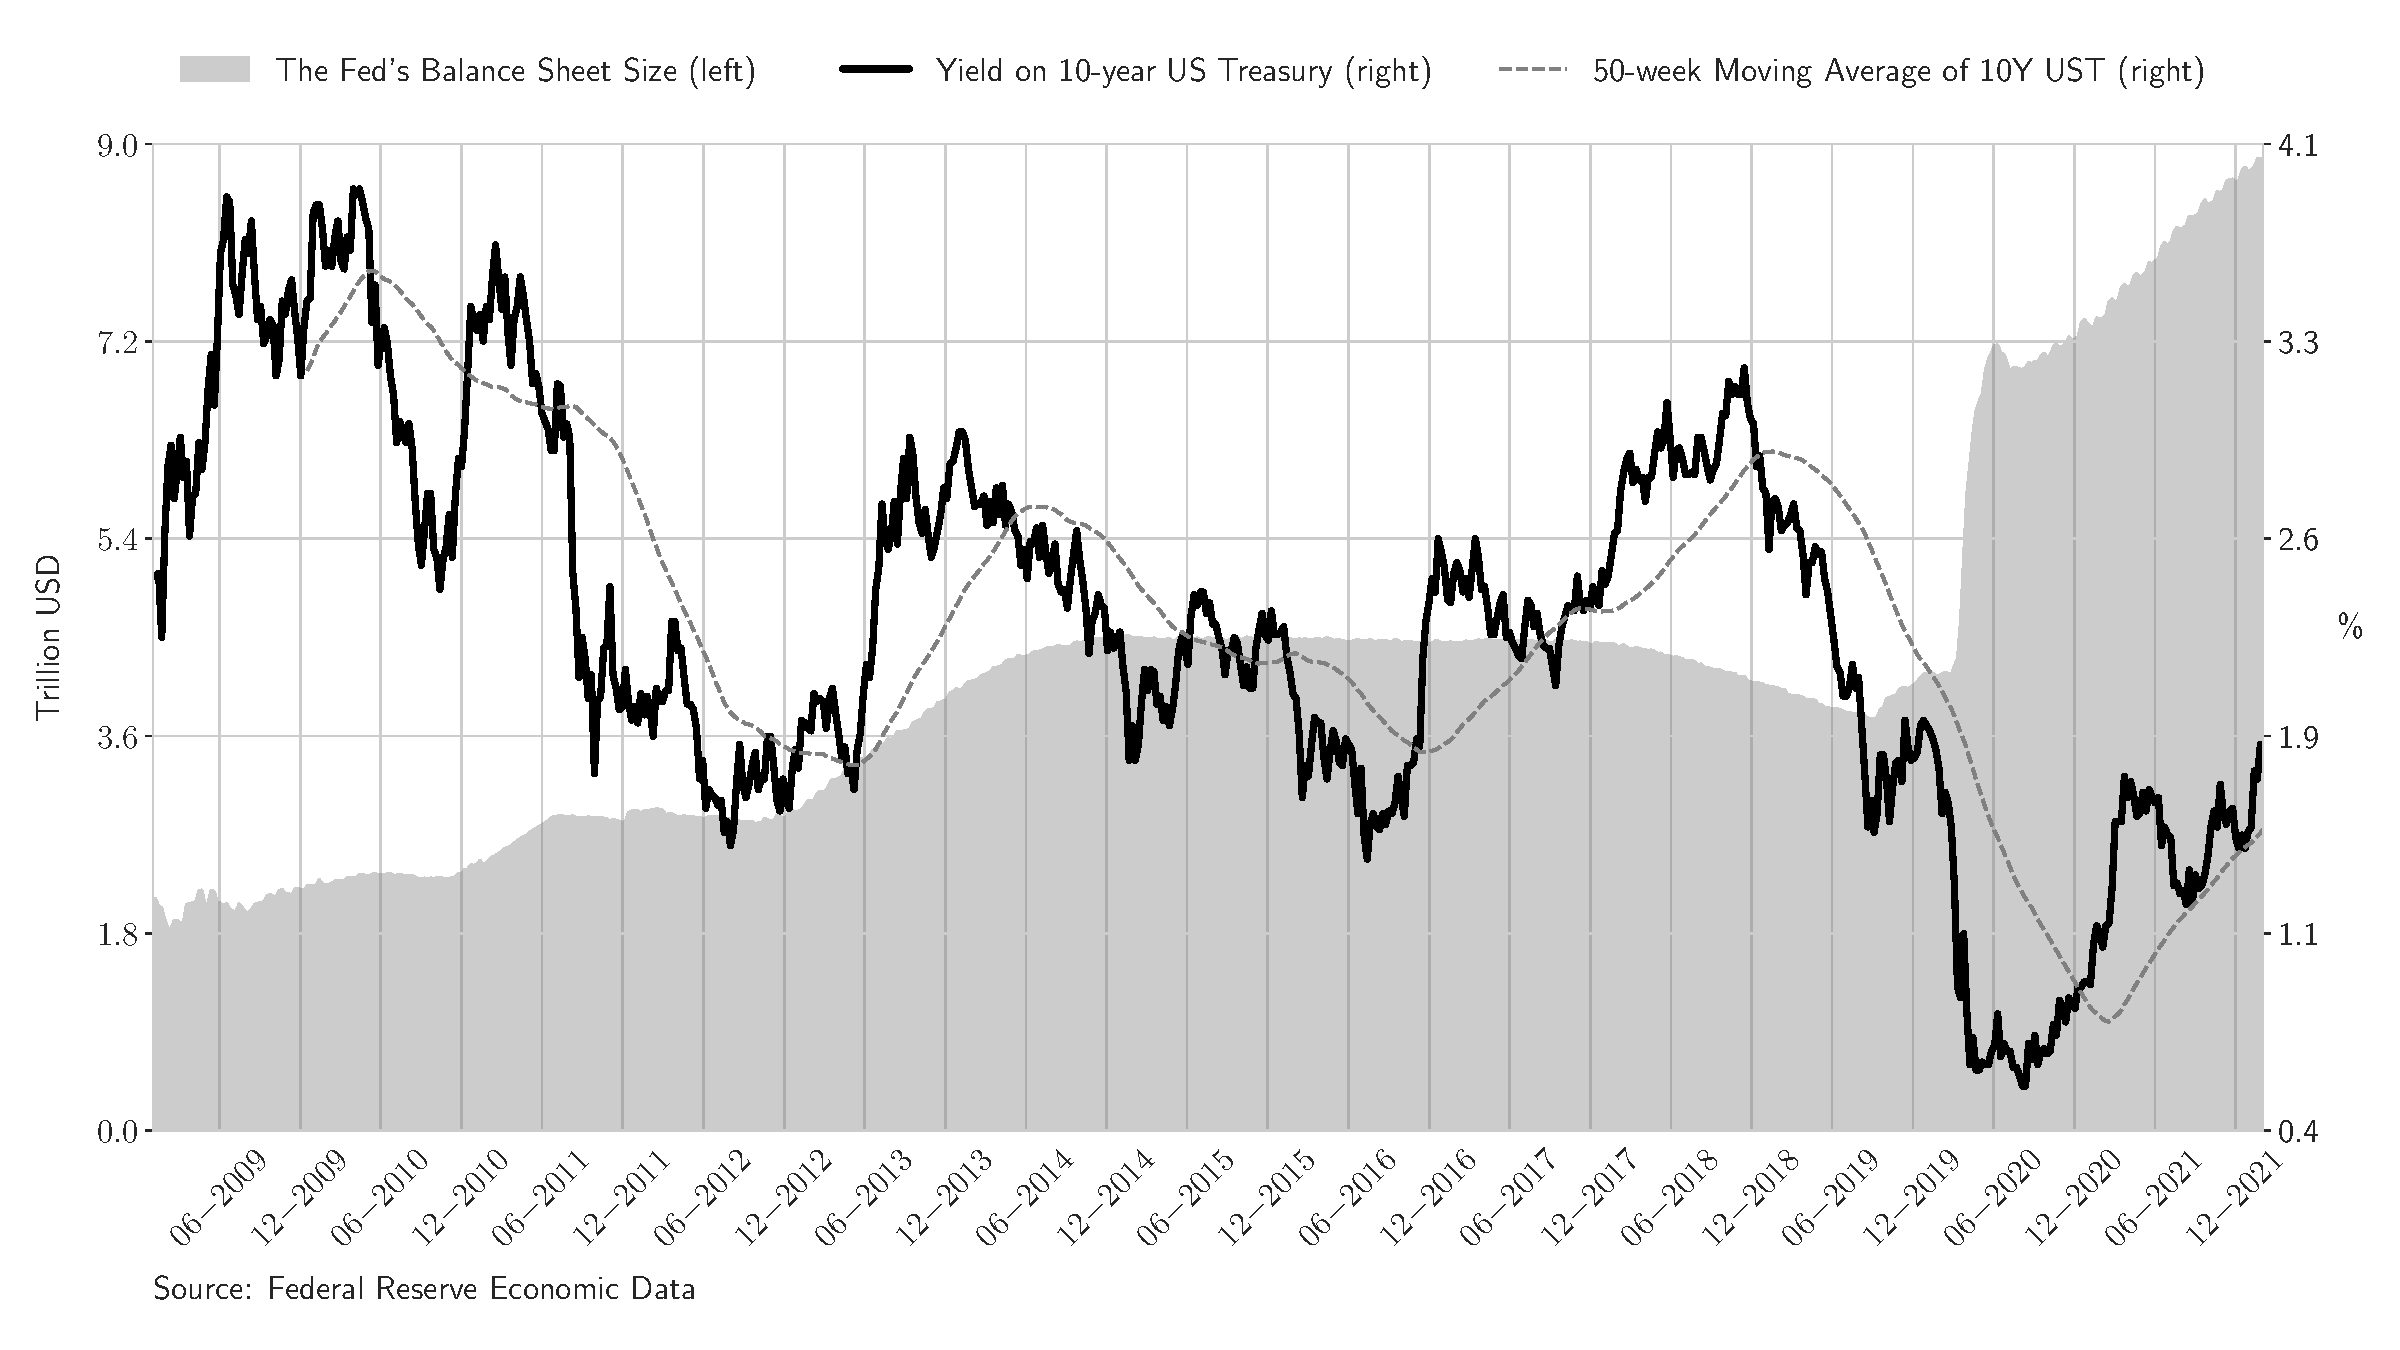
\includegraphics[width=0.99\linewidth]{fed_bs.pdf}
  \end{center}
  \label{Feds_BS}
\end{figure}


% Scarcity channel is one of the least studied effects of central bank large asset purchases. It is plausible that quantitative easing programs, by decreasing the supply of Treasuries, increase scarcity of these securities in the market, especially in the repo market. There has been some research done on scarcity channel by determining relationship between central bank asset purchases and special repo rates (Arrata et al., 2018; D'amico et al., 2014). The authors of both papers use a very detailed repo data to test the hypothesis of a central bank induced collateral shortage, however they don’t take into the account the mechanics of the collateral intermediation complex. Jank et al. (2020) look into the dynamics of the shadow banking system in the and link the re-use rate of collateral to the supply of collateral and repo rates in the Euro area. Nevertheless, there still is no evidence of the scarcity channel in US Treasury repo market, that considers off-balance sheet collateral creation. This research would investigate effects of quantitative easing in jjjjkthe US on the Treasury General Collateral repo rate, with the help of bank’s repledgedable collateral data that represents augmented “supply” of repo collateral endogenously created by the banking system itself.
%
% The idea is to use test causality with a simple OLS regression. The depended variable would be the overnight GC Treasury repo rate in one of three possible forms: a) repo rate in first-difference form1, b) fed funds upper target less repo rate, c) collateral spread, i.e. repo rate less unsecured rate, as in Nyborg and Rosel (2019).
% While Nyborg (2019) asks the question of what makes collateral spread to narrow and why does it often turn negative? Here, the main question is: does the central bank create

\newpage


% ----- COLLATERAL MECHANICS ----- 
\section{Mechanics of collateral}

\lipsum


% ----- COLLATERAL SHORTAGE ----- 
\section{Collateral shortage in years 2020-2022}

\lipsum


% ----- EMPIRICAL ----- 
\section{Empirical tests}

\subsection{Descriptive Statistics}

\lipsum

\subsection{Methodology}

\lipsum

\citet{nyborg2019a}

\subsection{Base Model}

\lipsum

\subsection{Extension}


\lipsum


% ----- CONCLUSIONS ----- 
\section{Conclusions}

\lipsum


% ----- APPENDIX (OPTIONAL) ----- 
%\newpage
% \appendix
% \noappendicestocpagenum
% \addappheadtotoc
% \appendixpage

% ----- BIBLIOGRAPHY ----- 
\newpage
\bibliography{refs}


% ----- STATEMENT ----- 
\newpage
\thispagestyle{firststyle}
\section*{Eidesstattliche Erklärung}
Der Verfasser erklärt an Eides statt, dass er die vorliegende Arbeit selbständig, ohne fremde Hilfe und ohne Benutzung anderer als die angegebenen Hilfsmittel angefertigt hat. Die aus fremden Quellen (einschliesslich elektronischer Quellen) direkt oder indirekt übernommenen Gedanken sind ausnahmslos als solche kenntlich gemacht. Die Arbeit ist in gleicher oder ähnlicher Form oder auszugsweise im Rahmen einer anderen Prüfung noch nicht vorgelegt worden.\\[2cm]

\hspace{60pt} 18.05.2022

\dotbox{Ort, Datum} \hfill \dotbox{Unterschrift des/der Verfassers/in}
\end{document}
